\documentclass[border=4pt,varwidth=6in]{standalone}
\usepackage[T1]{fontenc}
\usepackage{mathptmx}
\usepackage[scaled=0.92]{helvet}
\usepackage{courier}
\usepackage{setspace}
\usepackage{amsmath,amssymb,amsthm}
\usepackage{xcolor}
\usepackage{graphicx}
\usepackage{float}
\usepackage[font={singlespacing,normalsize},labelfont=bf,labelsep=period,justification=justified,singlelinecheck=false]{caption}
\usepackage{subcaption}
\usepackage{booktabs,multirow,longtable,threeparttable,array,tabularx}
\usepackage{enumitem}
%% preamble.tex — packages and macros shared by all chapters
% Engine compatibility: biber writes UTF-8 into the .bbl. Under pdfTeX, inputenc maps
% characters outside Latin-1 to T1 glyphs; under XeTeX (tectonic) they would be silently
% dropped from the 8-bit Times fonts, so map them explicitly.
\usepackage{iftex}
\ifXeTeX
  \usepackage{newunicodechar}
  \newunicodechar{č}{\v{c}}\newunicodechar{Č}{\v{C}}\newunicodechar{ě}{\v{e}}\newunicodechar{ř}{\v{r}}
  \newunicodechar{š}{\v{s}}\newunicodechar{Š}{\v{S}}\newunicodechar{ž}{\v{z}}\newunicodechar{Ž}{\v{Z}}
  \newunicodechar{Ł}{\L{}}\newunicodechar{ł}{\l{}}\newunicodechar{ń}{\'n}\newunicodechar{ś}{\'s}
  \newunicodechar{ć}{\'c}\newunicodechar{ż}{\.z}\newunicodechar{ź}{\'z}\newunicodechar{ę}{\k{e}}\newunicodechar{ą}{\k{a}}
  \newunicodechar{ő}{\H{o}}\newunicodechar{ű}{\H{u}}\newunicodechar{ğ}{\u{g}}\newunicodechar{ş}{\c{s}}\newunicodechar{ı}{\i}
\fi
\usepackage{physics}          % \ket, \bra, \expval, \dd, \abs, \norm
\usepackage{bm}
\usepackage{mathtools}
\usepackage{siunitx}
\sisetup{detect-all,per-mode=symbol,range-phrase=--,range-units=single}
\usepackage{tikz}
\usetikzlibrary{quantikz2}
\usetikzlibrary{arrows.meta,positioning,calc,shapes.geometric,fit,backgrounds,matrix,decorations.pathreplacing}
\usepackage{pgfplots}
\pgfplotsset{compat=1.18}
\usepgfplotslibrary{groupplots,fillbetween}
\usepackage[ruled,vlined,linesnumbered]{algorithm2e}
\SetAlFnt{\singlespacing\small}
% cleveref is loaded by ttuthesis.cls *before* algorithm2e, so its algorithm2e alias is never
% installed; name the algocf label type explicitly so \cref{alg:...} prints "Algorithm N".
\usepackage{listings}
\lstset{basicstyle=\ttfamily\footnotesize\singlespacing,breaklines=true,columns=fullflexible,
        keepspaces=true,frame=single,framerule=0.3pt,xleftmargin=1em,showstringspaces=false,
        commentstyle=\itshape\color{black!60},keywordstyle=\bfseries}
\lstdefinelanguage{qasm}{morekeywords={OPENQASM,include,qubit,bit,h,cx,rz,ry,measure,reset,barrier},sensitive=true,morecomment=[l]{//}}

% Theorem-like environments (numbered per chapter, Arabic chapter number)

% Color-blind-safe palette for plots (also varies markers/line styles: TTU accessibility rule)
\definecolor{cbBlue}{HTML}{0072B2}
\definecolor{cbOrange}{HTML}{E69F00}
\definecolor{cbGreen}{HTML}{009E73}
\definecolor{cbRed}{HTML}{D55E00}
\definecolor{cbPurple}{HTML}{CC79A7}
\definecolor{cbSky}{HTML}{56B4E9}
\definecolor{cbGray}{HTML}{555555}
\pgfplotscreateplotcyclelist{ttu}{%
  {cbBlue,mark=*,solid},{cbOrange,mark=square*,dashed},{cbGreen,mark=triangle*,dotted},
  {cbRed,mark=diamond*,dashdotted},{cbPurple,mark=pentagon*,densely dashed},{cbGray,mark=o,loosely dotted}}
\pgfplotsset{every axis/.append style={cycle list name=ttu,width=0.8\linewidth,height=0.5\linewidth,
  tick label style={font=\small},label style={font=\small},legend style={font=\footnotesize,cells={anchor=west}},
  grid=major,grid style={black!12}}}

% Domain macros
\newcommand{\qgear}{Q-GEAR}
\newcommand{\deal}{DEAL}
\newcommand{\qawa}{QAWA}
\newcommand{\qpie}{QPIE}
\newcommand{\vqt}{VQT}
\newcommand{\shardq}{ShardQ}
\newcommand{\nnqa}{NNQA}
\newcommand{\rubriq}{RubriQ}
\newcommand{\cudaq}{CUDA-Q}
\newcommand{\qiskit}{Qiskit}
\newcommand{\qcrank}{QCrank}
\newcommand{\bigO}[1]{\mathcal{O}\!\left(#1\right)}
\newcommand{\Hcost}{H_C}
\newcommand{\Hmix}{H_M}
\newcommand{\code}[3]{[[#1,#2,#3]]}
\newcommand{\eps}{\varepsilon}
\newcommand{\R}{\mathbb{R}}
\newcommand{\C}{\mathbb{C}}
\newcommand{\Z}{\mathbb{Z}}
% \Tr provided by physics
\DeclareMathOperator{\poly}{poly}
\DeclareMathOperator*{\argmin}{arg\,min}
\DeclareMathOperator*{\argmax}{arg\,max}

\newcommand{\todo}[1]{{\color{red!70!black}\textbf{[TODO: #1]}}}
\providecommand{\cref}[1]{#1}
\providecommand{\Cref}[1]{#1}
\providecommand{\labelcref}[1]{#1}
\providecommand{\ref}[1]{#1}
\providecommand{\cite}[1]{[#1]}
\begin{document}
\begin{figure}[H]
\centering
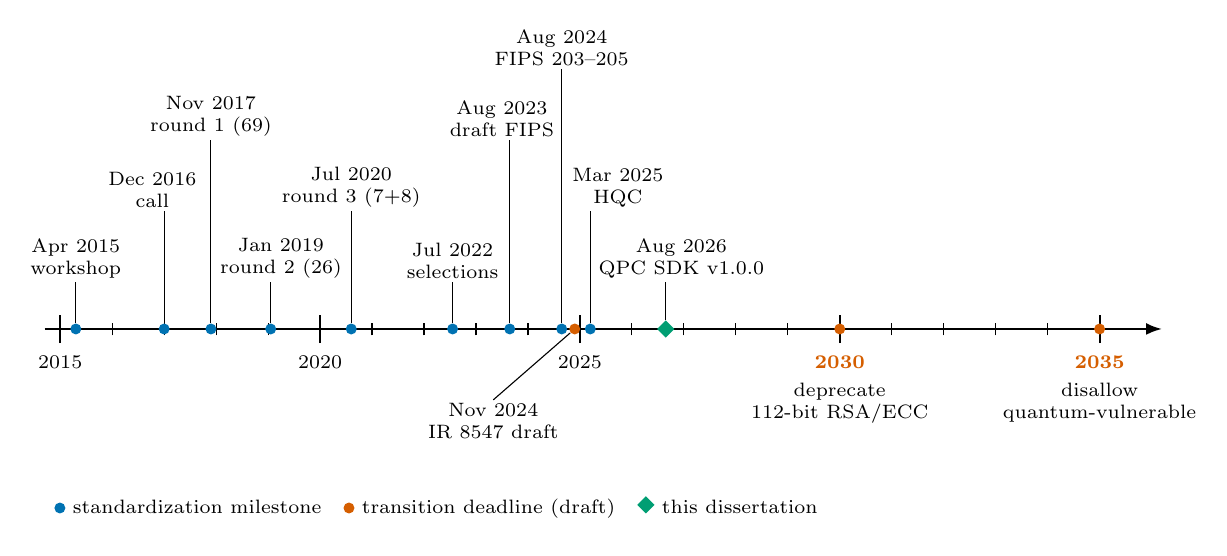
\begin{tikzpicture}[x=6.6mm,y=1mm,font=\scriptsize,
  up/.style={anchor=south,align=center,inner sep=1pt},
  dn/.style={anchor=north,align=center,inner sep=1pt},
  ev/.style={circle,fill=cbBlue,inner sep=1.4pt},
  dl/.style={circle,fill=cbRed,inner sep=1.4pt},
  us/.style={diamond,fill=cbGreen,inner sep=1.6pt}]
  \draw[thick,-{Latex[length=2mm]}] (-0.3,0) -- (21.2,0);
  \foreach \yr in {2015,...,2035}{ \pgfmathsetmacro{\xx}{\yr-2015} \draw (\xx,-0.8) -- (\xx,0.8); }
  \foreach \yr in {2015,2020,...,2035}{ \pgfmathsetmacro{\xx}{\yr-2015} \draw[thick] (\xx,-1.8) -- (\xx,1.8); }
  \foreach \yr in {2015,2020,2025}{ \pgfmathsetmacro{\xx}{\yr-2015} \node[dn] at (\xx,-3) {\yr}; }
  \node[ev] (a) at (0.3,0) {};   \draw (a) -- (0.3,6);    \node[up] at (0.3,6)   {Apr 2015\\ workshop};
  \node[ev] (b) at (2.0,0) {};   \draw (b) -- (2.0,15);   \node[up,xshift=-1.5mm] at (2.0,15) {Dec 2016\\ call};
  \node[ev] (c) at (2.9,0) {};   \draw (c) -- (2.9,24);   \node[up] at (2.9,24)  {Nov 2017\\ round 1 (69)};
  \node[ev] (d) at (4.05,0) {};  \draw (d) -- (4.05,6);   \node[up,xshift=1.3mm] at (4.05,6) {Jan 2019\\ round 2 (26)};
  \node[ev] (e) at (5.6,0) {};   \draw (e) -- (5.6,15);   \node[up] at (5.6,15)  {Jul 2020\\ round 3 (7+8)};
  \node[ev] (f) at (7.55,0) {};  \draw (f) -- (7.55,6);   \node[up] at (7.55,6)  {Jul 2022\\ selections};
  \node[ev] (g) at (8.65,0) {};  \draw (g) -- (8.65,24);  \node[up,xshift=-1mm] at (8.65,24) {Aug 2023\\ draft FIPS};
  \node[ev] (h) at (9.65,0) {};  \draw (h) -- (9.65,33);  \node[up] at (9.65,33) {Aug 2024\\ FIPS 203--205};
  \node[ev] (i) at (10.2,0) {};  \draw (i) -- (10.2,15);  \node[up,xshift=3.5mm] at (10.2,15) {Mar 2025\\ HQC};
  \node[us] (j) at (11.65,0) {}; \draw (j) -- (11.65,6);  \node[up,xshift=2mm] at (11.65,6) {Aug 2026\\ QPC SDK v1.0.0};
  \node[dl] (k) at (9.9,0) {};   \draw (k) -- (55mm,-9);  \node[dn] at (55mm,-9) {Nov 2024\\ IR 8547 draft};
  \node[dl] (l) at (15,0) {};    \node[dn,text=cbRed,font=\scriptsize\bfseries] at (15,-3) {2030}; \node[dn] at (15,-6.4) {deprecate\\ 112-bit RSA/ECC};
  \node[dl] (m) at (20,0) {};    \node[dn,text=cbRed,font=\scriptsize\bfseries] at (20,-3) {2035}; \node[dn] at (20,-6.4) {disallow\\ quantum-vulnerable};
  \node[anchor=north west,align=left] at (-0.3,-20) {\tikz\node[ev]{}; standardization milestone\quad \tikz\node[dl]{}; transition deadline (draft)\quad \tikz\node[us]{}; this dissertation};
\end{tikzpicture}
\end{figure}
\end{document}
